\documentclass[11pt, a4paper]{article}
\usepackage{pdfpages}
\usepackage{parallel}
\usepackage[T2A]{fontenc}
%\usepackage{ucs}
\usepackage[utf8]{inputenc}
\usepackage[english,russian]{babel}
\usepackage{hyperref}
\usepackage{rotating}
\usepackage[inner=2cm,top=1.8cm,outer=2cm,bottom=2.3cm,nohead]{geometry}
%\usepackage{listings}
\usepackage{graphicx}
\usepackage{wrapfig}
\usepackage{longtable}
\usepackage{indentfirst}
\usepackage{array}
\usepackage{tikzsymbols}
\usepackage{soul}
\usepackage[ruled,vlined]{algorithm2e}
\usepackage{qrcode}
\counterwithout{figure}{section} 

\usepackage{url}
\makeatletter
\g@addto@macro{\UrlBreaks}{\UrlOrds}
\makeatother

\newcolumntype{P}[1]{>{\raggedright\arraybackslash}p{#1}}
\frenchspacing
%\usepackage{fixltx2e} %text sub- and superscripts
\usepackage{icomma} % коскі ў матэматычным рэжыме
%\PreloadUnicodePage{4}

\newcommand{\longpage}{\enlargethispage{\baselineskip}}
\newcommand{\shortpage}{\enlargethispage{-\baselineskip}}

\def\switchlang#1{\expandafter\csname switchlang#1\endcsname}
\def\switchlangbe{
\let\saverefname=\refname%
\def\refname{Літаратура}%
\def\figurename{Іл.}%
}
\def\switchlangru{
\let\saverefname=\refname%
\let\savefigurename=\figurename%
\def\refname{Литература}%
\def\figurename{Рис.}%
}
\def\switchlangen{
\let\saverefname=\refname%
\def\refname{References}%
\def\figurename{Fig.}%
}

\hyphenation{admi-ni-stra-tive}
\hyphenation{ex-pe-ri-ence}
\hyphenation{fle-xi-bi-li-ty}
\hyphenation{Py-thon}
\hyphenation{ma-the-ma-ti-cal}
\hyphenation{re-ported}
\hyphenation{imp-le-menta-tions}
\hyphenation{pro-vides}
\hyphenation{en-gi-neering}
\hyphenation{com-pa-ti-bi-li-ty}
\hyphenation{im-pos-sible}
\hyphenation{desk-top}
\hyphenation{elec-tro-nic}
\hyphenation{com-pa-ny}
\hyphenation{de-ve-lop-ment}
\hyphenation{de-ve-loping}
\hyphenation{de-ve-lop}
\hyphenation{da-ta-ba-se}
\hyphenation{plat-forms}
\hyphenation{or-ga-ni-za-tion}
\hyphenation{pro-gramming}
\hyphenation{in-stru-ments}
\hyphenation{Li-nux}
\hyphenation{sour-ce}
\hyphenation{en-vi-ron-ment}
\hyphenation{Te-le-pathy}
\hyphenation{Li-nux-ov-ka}
\hyphenation{Open-BSD}
\hyphenation{Free-BSD}
\hyphenation{men-ti-on-ed}
\hyphenation{app-li-ca-tion}

\def\progref!#1!{\texttt{#1}}
\renewcommand{\arraystretch}{2} %Іначай формулы ў матрыцы зліпаюцца з лініямі
\usepackage{array}

\def\interview #1 (#2), #3, #4, #5\par{

\section[#1, #3, #4]{#1 -- #3, #4}
\def\qname{LVEE}
\def\aname{#1}
\def\q ##1\par{{\noindent \bf \qname: ##1 }\par}
\def\a{{\noindent \bf \aname: } \def\qname{L}\def\aname{#2}}
}

\def\interview* #1 (#2), #3, #4, #5\par{

\section*{#1\\{\small\rm #3, #4. #5}}
\ifx\ParallelWhichBox\undefined%
    \addcontentsline{toc}{section}{#1, #3, #4}%
\else%
\ifnum\ParallelWhichBox=0%
    \addcontentsline{toc}{section}{#1, #3, #4}%
\fi\fi%

\def\qname{LVEE}
\def\aname{#1}
\def\q ##1\par{{\noindent \bf \qname: ##1 }\par}
\def\a{{\noindent \bf \aname: } \def\qname{L}\def\aname{#2}}
}

\newcommand{\interviewfooter}[1]{
\vskip 1em
\noindent \textit{#1}
}

\AtEndDocument{\vfill\centering \qrcode{https://github.com/fiowro/mouses/blob/main/\jobname.pdf}}

\switchlang{ru}
\begin{document}

\title{1985 "--- Microsoft Gray-eyed Mouse}
\date{}
\maketitle
\selectlanguage{russian}

Данная мышь, появившаяся в продаже в 1985 году, стала вторым поколением мышей Microsoft. Компания просто называла свои ранние модели <<мышь Microsoft>>, иногда уточняя ещё способ подключения к компьютеру. Поэтому официальное название данного экземпляра <<Microsoft Serial Mouse>> скорее запутывало, и мышь получила известность среди пользователей под названием <<Cероглазой мыши Microsoft>> (чтобы дифференцировать ее от мыши первого поколения с парой зеленых кнопок, подаривших ей название <<Зеленоглазая мышь>>). Также иногда эту мышь упоминают под названием <<Microsoft Mouse 5.0>> \cite{mouses}, очевидно из-за вариантов мышей первого поколения с разными интерфейсами. Производством мыши, как и в случае первого поколения, занималась японская компания Alps.

\begin{figure}[h]
   \centering
    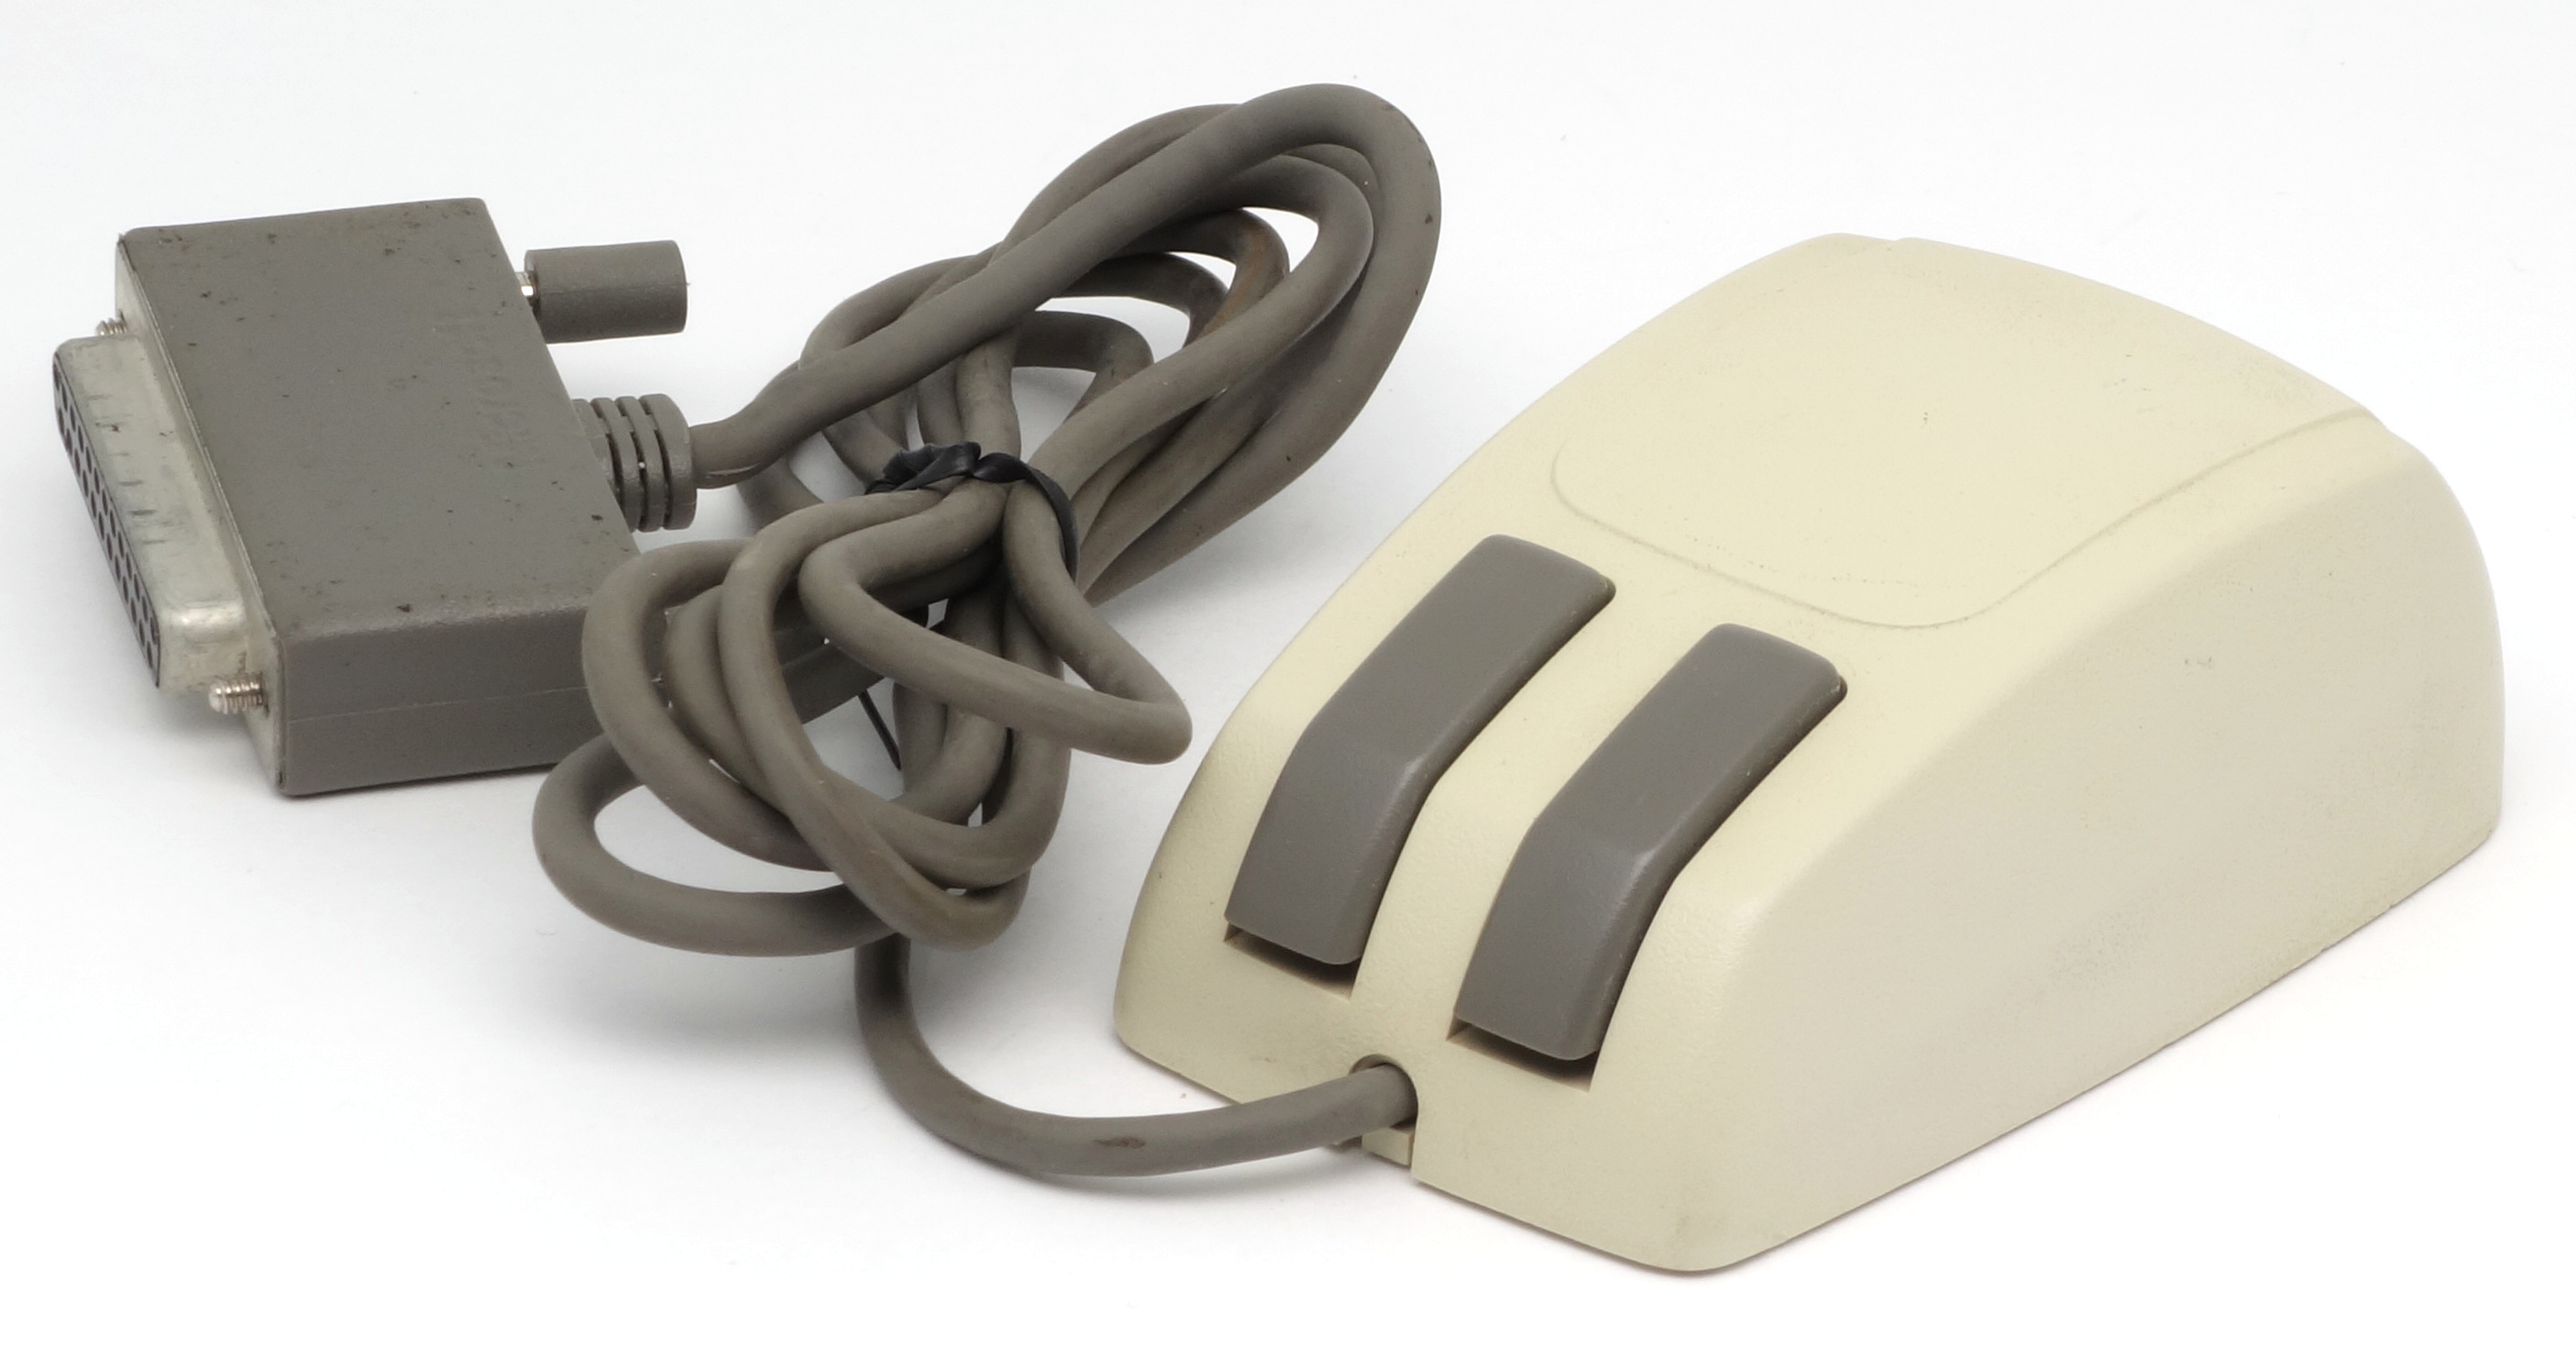
\includegraphics[scale=0.5]{1985_microsoft_gray_eyed_mouse/pic_30.jpg}
    \caption{Microsoft Gray-eyed Mouse}
    \label{fig:MicrosoftGrayEyedPic}
\end{figure}

Второе поколение получило несколько существенных улучшений как в конструкции, так и в плане эргономики. Материалом корпуса стал классический бежевый пластик, а сам корпус стал более выпуклым. Две контрастные серые кнопки по-прежнему расположены на наклонной передней грани, но заходят также и на верхнюю стенку корпуса (рис.  \ref{fig:MicrosoftGrayEyedPic}). Нужно отметить, что иногда встречаются также экземпляры <<сероглазой>> мыши с кнопками красного цвета.

Нижняя часть содержит стальной шар с резиновым покрытием и фиксирующее кольцо, которое можно сдвинуть в сторону, чтобы извлечь шар для чистки мыши (рис. \ref{fig:MicrosoftGrayEyedTopAndBottom}).

\begin{figure}[h]
    \centering
    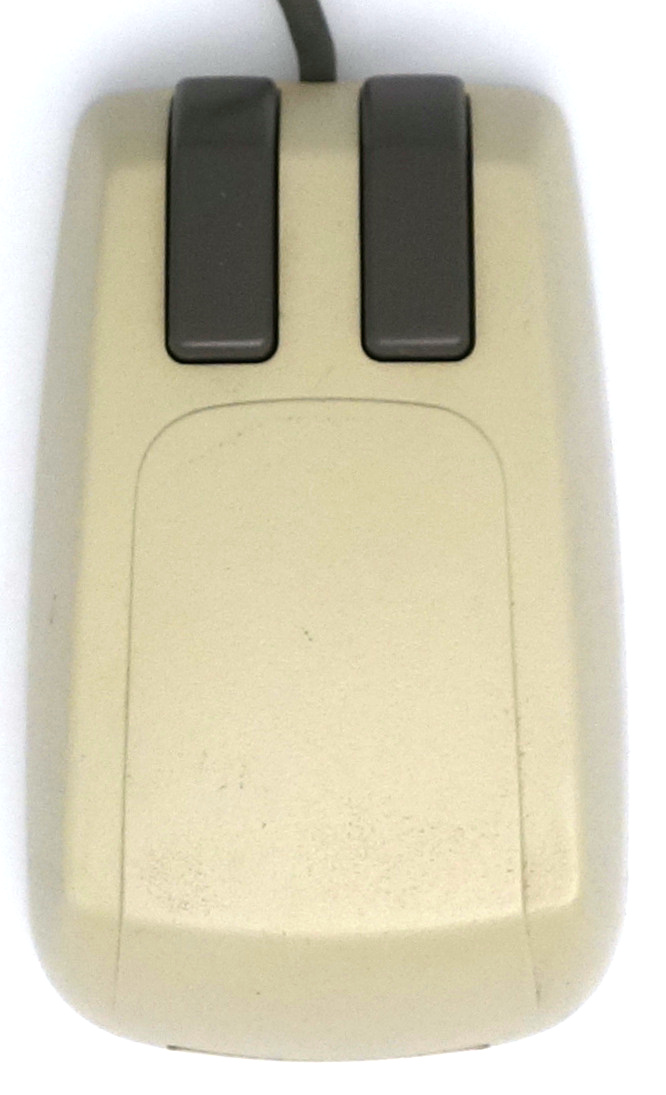
\includegraphics[scale=0.55]{1985_microsoft_gray_eyed_mouse/top_30.jpg}
    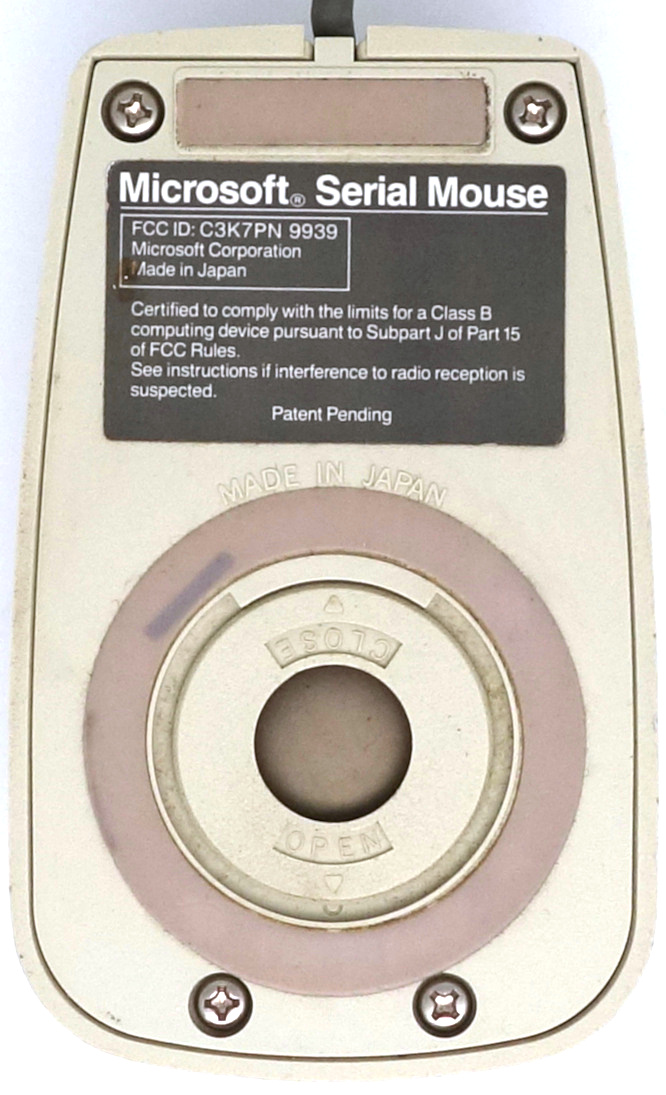
\includegraphics[scale=0.55]{1985_microsoft_gray_eyed_mouse/bottom_30.jpg}
    \caption{Microsoft Gray-eyed Mouse, вид сверху и снизу}
    \label{fig:MicrosoftGrayEyedTopAndBottom}
\end{figure}

Вокруг фиксирующего кольца наблюдается контрастная кольцеобразная накладка из низкофрикционного материала, являющаяся отличительной чертой многих мышей 80-х годов, разработанных в Японии. Резиновое покрытие шара дало мыши существенное преимущество по сравнению с обычным стальным шаром зеленоглазой мыши: оно одновременно уменьшало проскальзывание шара и обеспечивало тихую работу мыши на твердых поверхностях.

\begin{figure}[h]
    \centering
    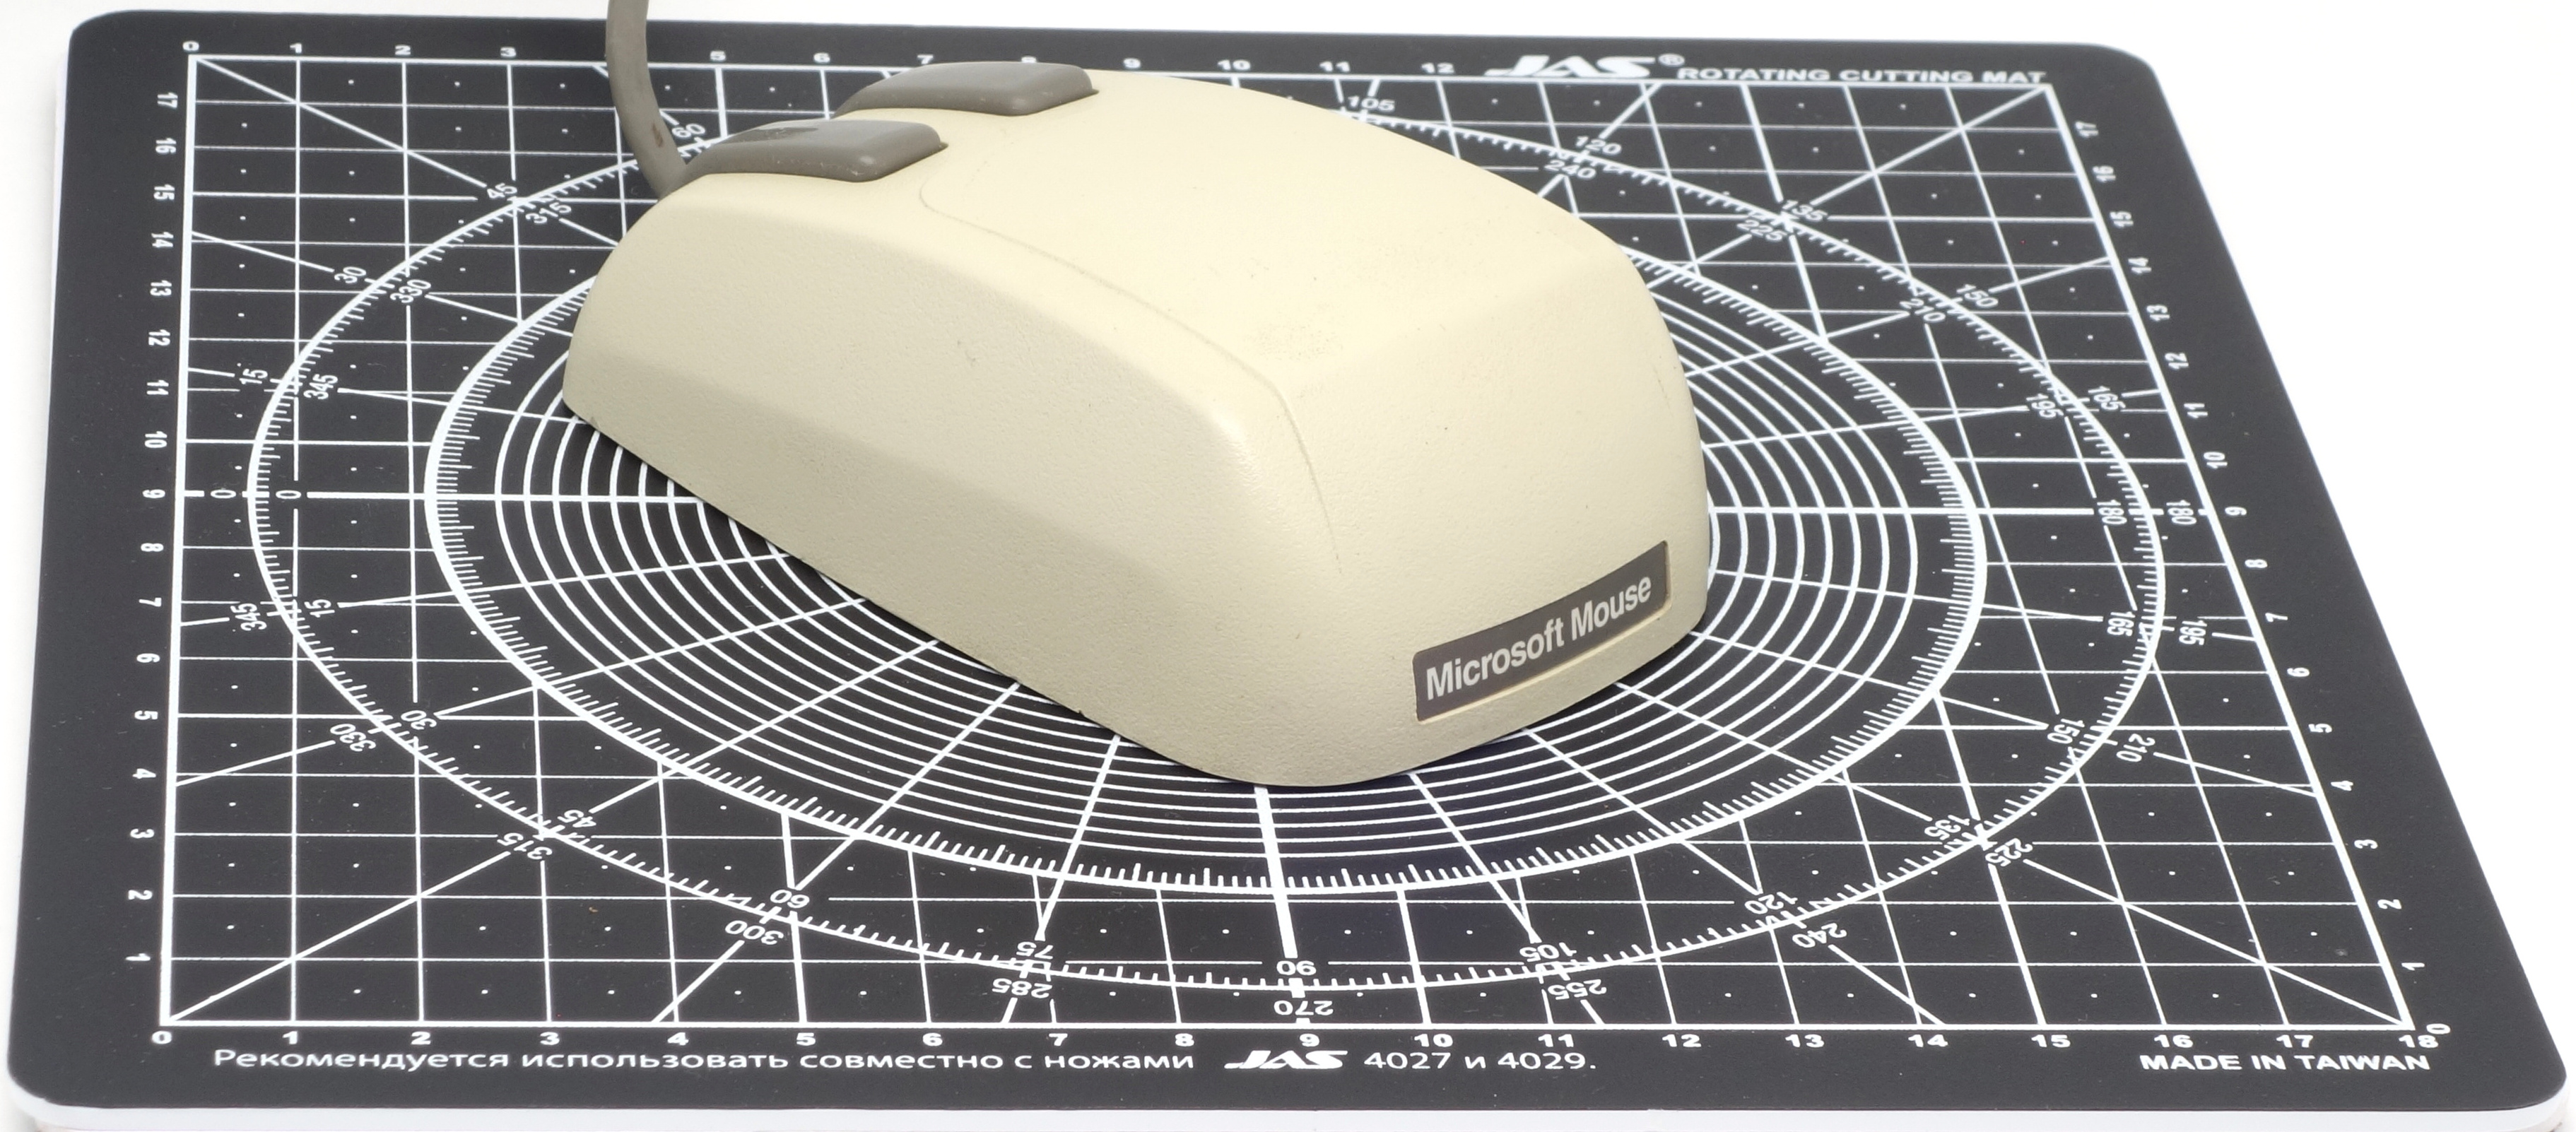
\includegraphics[scale=0.5]{1985_microsoft_gray_eyed_mouse/size_30.jpg}
    \caption{Microsoft Gray-eyed Mouse на размерном коврике с шагом сетки 1~см}
    \label{fig:MicrosoftGrayEyedSize}
\end{figure}

Размеры мыши являются типичными для 80-х годов (рис. \ref{fig:MicrosoftGrayEyedSize}) и определяются размерами типового узла ALPS. В рекламных материалах Microsoft упоминается, что <<огибающие корпус командные кнопки спроектированы таким образом, чтобы естественно помещаться в ладони любого размера>> \cite{mouses}. Часть критики в адрес эргономики мышей первого поколения касалась возможности сдвинуть мышь, нажимая кнопки на передней стенке корпуса, и такое двойное положение кнопок, очевидно, решало данную проблему, позволяя нажимать на них сверху тем, кому это удобнее (рис. \ref{fig:MicrosoftGrayEyedHand}). Вслед за Microsoft, эта угловая форма кнопок появилась в некоторых других мышах. Больше всего сходства, вплоть до похожей формы корпуса, демонстрируют мыши ProCorp Serial Mouse 1988 года выпуска и Vatek Сolor Mouse 1989 года.

\begin{figure}[h]
    \centering
    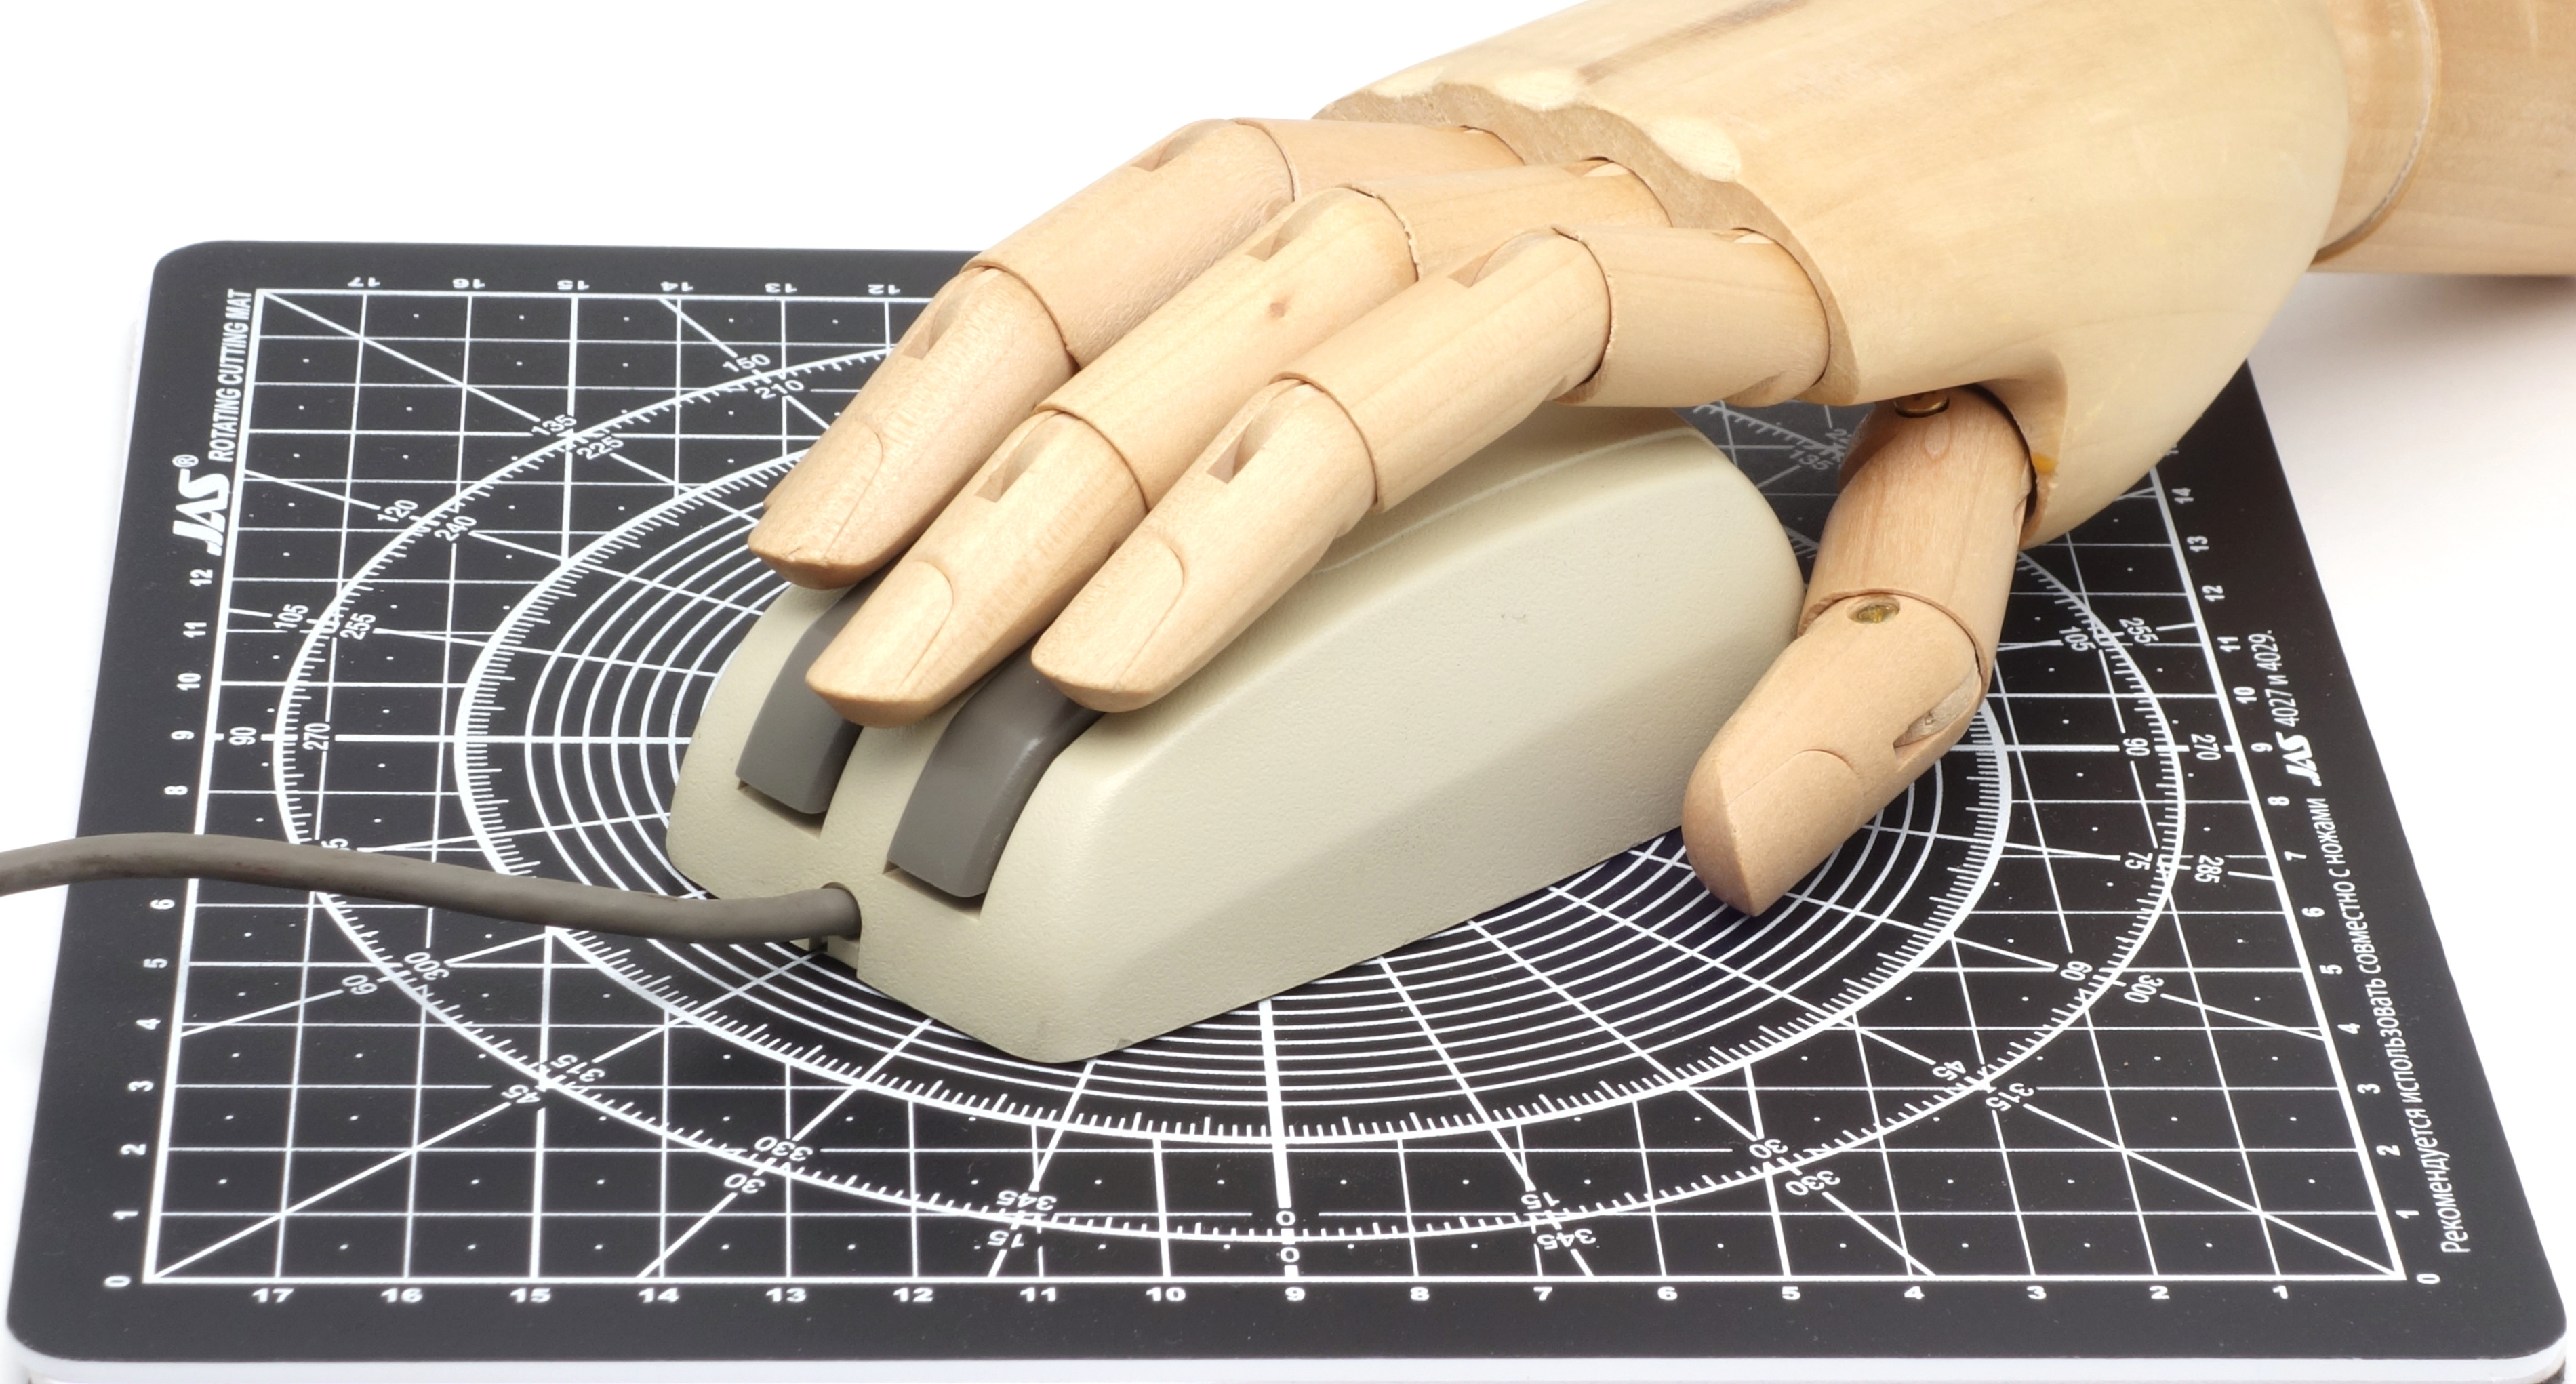
\includegraphics[scale=0.5]{1985_microsoft_gray_eyed_mouse/hand_30.jpg}
    \caption{Microsoft Gray-eyed Mouse с моделью руки человека}
    \label{fig:MicrosoftGrayEyedHand}
\end{figure}

Также рекламные материалы отмечали <<вдвое большее разрешение, чем у большинства других мышей, "--- 200 точек на дюйм>> (под <<большинством других мышей>> в данном случае имелось в виду первое поколение мышей Microsoft).

Данный экземпляр мыши имеет последовательный интерфейс подключения. Кроме того эта модель выпускалась как квадратурная мышь в двух вариантах \cite{guide}: с шинным интерфейсом (в комплекте со специальной платой-адаптером для установки в системный блок) и с интерфейсом InPort (ставшим попыткой Microsoft стандартизировать интерфейс подключения квадратурных мышей,  соответсвующие адаптеры и переходники для них). При этом у первых двух поколений мышей Microsoft с последовательным интерфейсом совпадает код FCC ID, поэтому на рис. \ref{fig:MicrosoftGrayEyedTopAndBottom} можно видеть FCC ID <<зелоноглазой>> мыши, зарегистрированный в 1983 году \cite{zero}.

\begin{figure}[h]
    \centering
    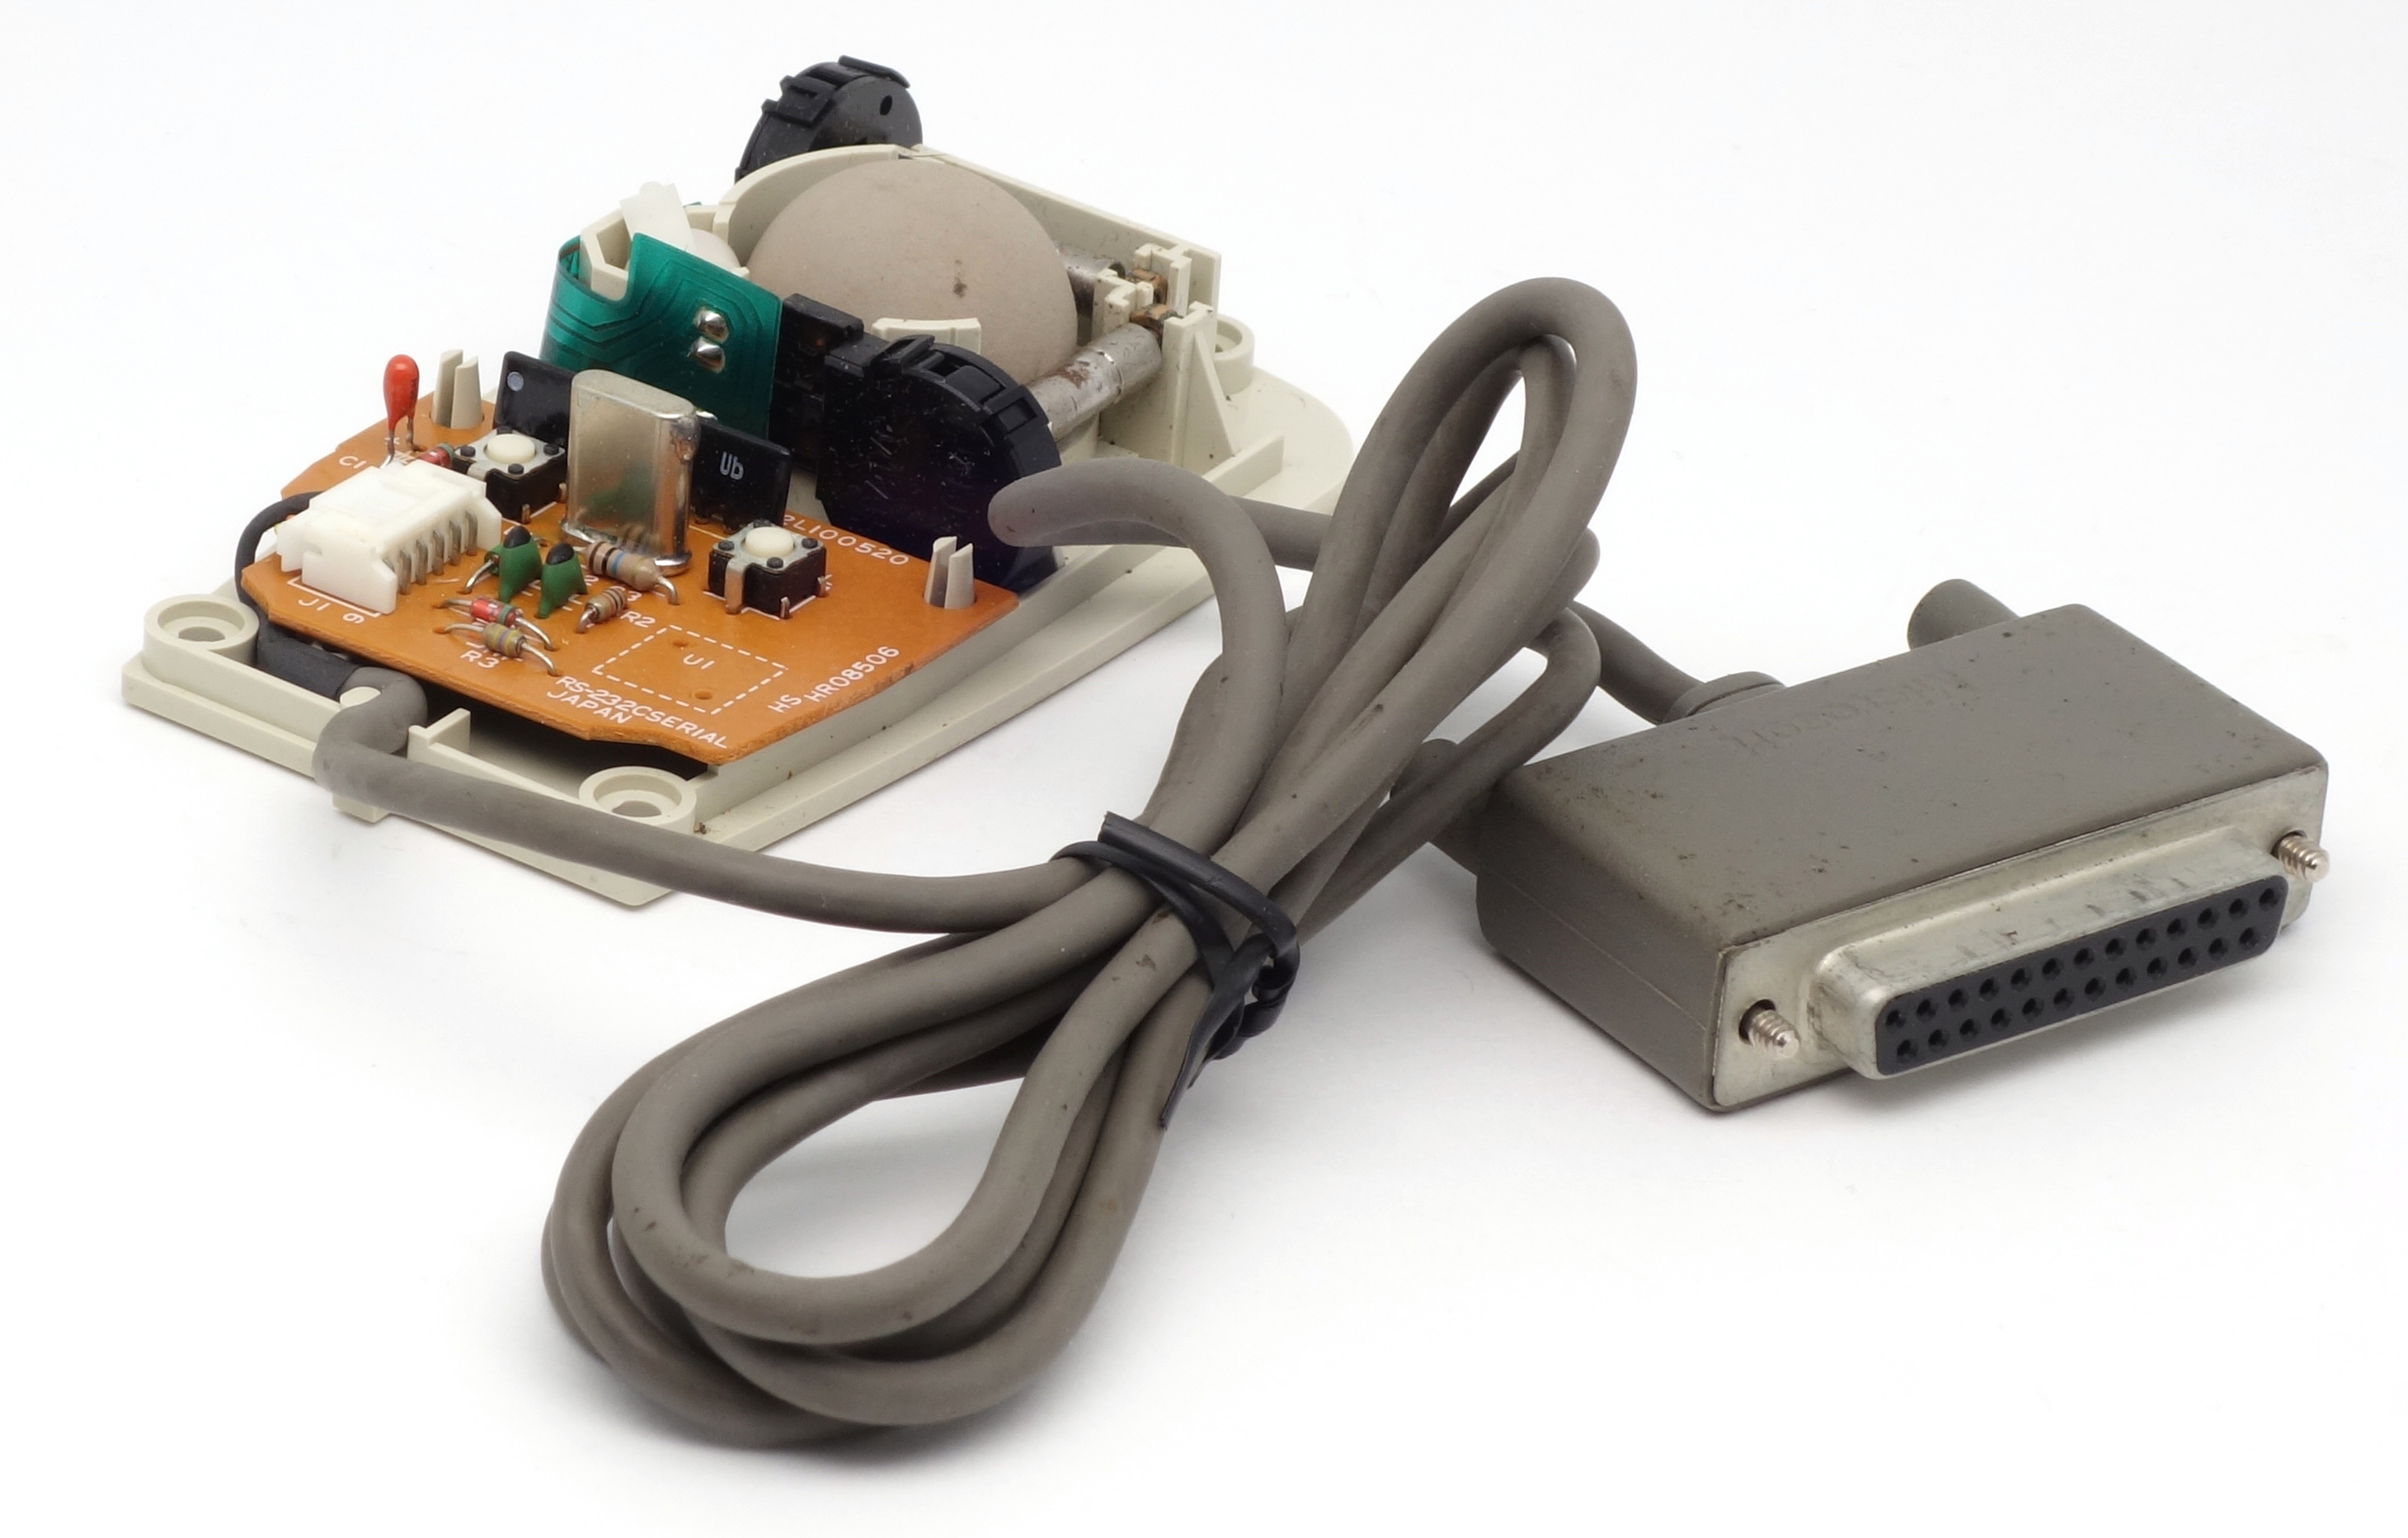
\includegraphics[scale=0.5]{1985_microsoft_gray_eyed_mouse/inside_30.jpg}
    \caption{Microsoft Gray-eyed Mouse в разобранном виде}
    \label{fig:MicrosoftGrayEyedInside}
\end{figure}

Внутреннее устройство мыши показано на рис. \ref{fig:MicrosoftGrayEyedInside}. Очевидно, реальным изготовителем мыши была японская компания Alps, часто выступавшая подрядчиком в разработке мышей по заказу других фирм (услугами Alps в частности пользовались такие компании, как IBM, Sharp, NeXT,  Siemens, Intergraph). Alps обычно изготавливала для каждого заказчика дизайн мыши с уникальной формой корпуса и расположением кнопок, но использовала одно и то же конструктивное исполнение в нескольких устройствах. В частности, данная мышь совпадает (включая нижнюю часть корпуса, массивные металлические ролики с подшипниками, узел регистрации движенияна основе закрытых контактных энкодеров, подключенный T-образным гибким шлейфом к двусторонней печатной плате) с продававшейся в 1986 году мышью Panasonic FS-JM650 и с IBM PS/2 Mouse, выпущенной в 1987 году.

\begin{thebibliography}{9}
\bibitem{mouses} Microsoft Gray-eyed Mouse \url{https://web.archive.org/web/20210417233303/http://oldmouse.com/mouse/microsoft/grayeyed.shtml}
\bibitem{guide} Microsoft Mouse User Guide. Microsoft, 1986. \url{https://minuszerodegrees.net/manuals/Microsoft/Microsoft%20Mouse%20-%20User's%20Guide%20-%201986.pdf}
\bibitem{zero} Microsoft Mouse. Minus zero degrees \url{https://www.minuszerodegrees.net/msmouse/Microsoft%20mouse.htm}
\end{thebibliography}
\end{document}
